\newprob{1715325454}
{
    一輛汽車在一條直路上行駛。下圖所示為汽車的 位移$s$隨時間$t$的變化。
    \par{\par\centering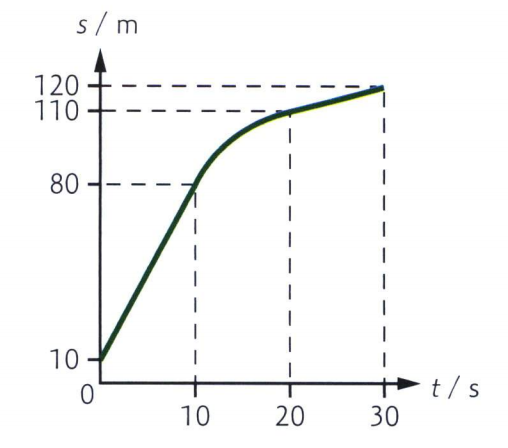
\includegraphics[width=.5\textwidth]{./img/ch45prob_2024-05-10-15-17-53.png}\par}
    \begin{parts}
        \part 描述汽車在$t=0$至 \qty{30}{s} 的運動。\zzh{2}
        \dlines{2}
        \clearpage
        \part 求汽車在$t=0$至\qty{30}{s} 間的平均速度。\zzh{2}
        \dlines{2}
        \begin{subparts}
            \subpart 123
            \subpart djiejdiowe
        \end{subparts}
    \end{parts}
}{}

\newprob{1715325820}
{
    在光滑表面上,兩磚方塊P和Q並排而立,而兩 者之中以P的質量較大。一個量值為F的水平 力,分別以圖a和b所示的方式作用在方塊上。
    \par{\par\centering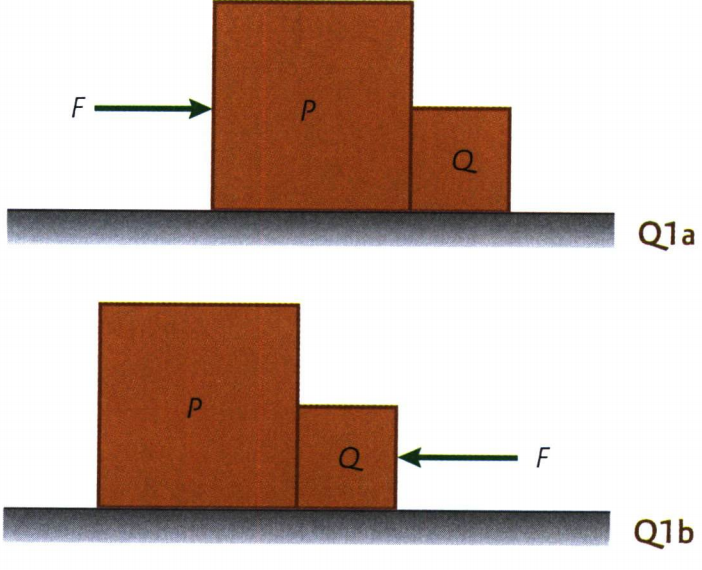
\includegraphics[width=.4\textwidth]{./img/ch45prob_2024-05-10-15-31-16.png}\par}
    \begin{statements}
        \task 方塊P的加速度
        \task  方塊P所受的淨力
        \task 方塊P作用在方塊Q上的力
    \end{statements}
    \begin{tasks}(2)
        \task 只有(1)和(2)
        \task 只有(1)和(3)
        \task 只有(2)和(3)
        \task (1), (2) 和 (3)
    \end{tasks}

}{A}

\newprob{1715327072}
{
    一磚方塊受力$F$作 用,力$F$與水平表面成夾角$\theta$。
    \par{\par\centering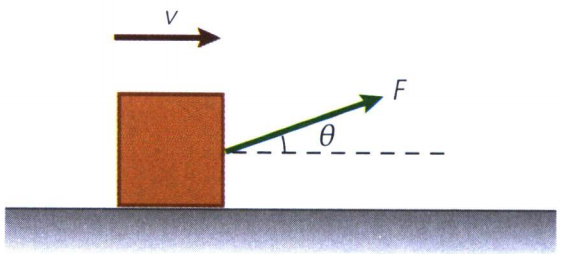
\includegraphics[width=.4\textwidth]{./img/ch45prob_2024-05-10-15-45-36.png}\par}
    方塊以匀速度$v$沿水平表面移動,期間受一道阻 力作用。設$R$、$W$ 和$f$分別為作用在方塊上的法 向反作用力、重量和摩擦力。下列哪一幅圖正確 展示作用在方塊上的力?
    \begin{tasks}(2)
        \task \topalign{\par\centering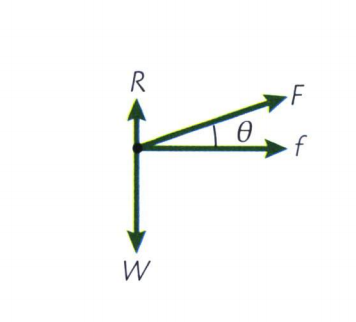
\includegraphics[width=.25\textwidth]{./img/ch45prob_2024-05-10-15-47-21.png}\par}
        \task \topalign{\par\centering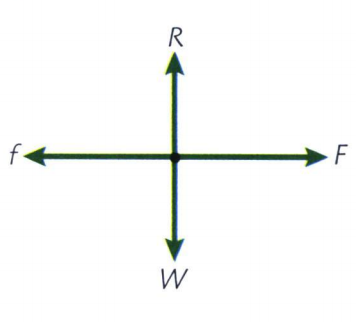
\includegraphics[width=.25\textwidth]{./img/ch45prob_2024-05-10-15-47-47.png}\par}
        \task \topalign{\par\centering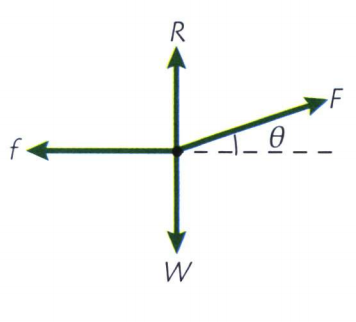
\includegraphics[width=.25\textwidth]{./img/ch45prob_2024-05-10-15-47-37.png}\par}
        \task \topalign{\par\centering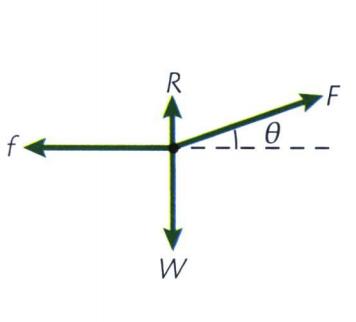
\includegraphics[width=.25\textwidth]{./img/ch45prob_2024-05-10-15-47-57.png}\par}
    \end{tasks}

}{}